\documentclass[11pt]{article}

% ---------------------------------------------------------------
% INFO 579 -- Project 1: Requirements Analysis
% Compile with: pdflatex requirements_analysis.tex   (run twice)
% ---------------------------------------------------------------

\usepackage[letterpaper,margin=0.75in]{geometry}
\usepackage[T1]{fontenc}
\usepackage[utf8]{inputenc}
\usepackage{charter}
\usepackage[scaled=0.92]{helvet}
\usepackage[table]{xcolor}
\usepackage{longtable}
\usepackage{graphicx}
\graphicspath{{img/}}
\usepackage{array}
\usepackage{ragged2e}
\usepackage{titlesec}
\usepackage{microtype}
\usepackage{needspace}
\usepackage{enumitem}
\usepackage{multicol}
\usepackage[colorlinks=true,urlcolor=headblue,linkcolor=black,citecolor=black]{hyperref}

\definecolor{hdrgray}{HTML}{E8E8E8}
\definecolor{headblue}{HTML}{2E74B5}
\definecolor{rulegray}{HTML}{BFBFBF}

\titleformat{\section}{\color{headblue}\sffamily\Large\bfseries}{}{0pt}{}
\titlespacing*{\section}{0pt}{16pt}{8pt}
\titleformat{\subsection}{\color{headblue}\sffamily\large\bfseries}{}{0pt}{}
\titlespacing*{\subsection}{0pt}{12pt}{4pt}

\setlength{\parindent}{0pt}
\setlength{\parskip}{6pt}
\setlength{\arrayrulewidth}{0.4pt}
\arrayrulecolor{rulegray}
\renewcommand{\arraystretch}{1.25}

% Fixed-width, vertically centred column
\newcolumntype{M}[1]{>{\RaggedRight\arraybackslash}m{#1}}
% Fixed-width justified column
\newcolumntype{L}[1]{>{\RaggedRight\arraybackslash}p{#1}}
% Same, never hyphenated (data type cells)
\newcolumntype{T}[1]{>{\RaggedRight\hyphenpenalty=10000\exhyphenpenalty=10000\arraybackslash}p{#1}}
% Quoted ENUM member
\newcommand{\q}[1]{\textquotesingle#1\textquotesingle}

% Column widths for the five-column entity tables
\newlength{\colA}\setlength{\colA}{1.50in}
\newlength{\colB}\setlength{\colB}{1.45in}
\newlength{\colC}\setlength{\colC}{0.85in}
\newlength{\colD}\setlength{\colD}{0.85in}
\newlength{\colE}\setlength{\colE}{1.30in}
% Full span across all five columns (widths + 8 x \tabcolsep + 4 x \arrayrulewidth)
\newlength{\colFull}
\setlength{\colFull}{\colA}
\addtolength{\colFull}{\colB}\addtolength{\colFull}{\colC}
\addtolength{\colFull}{\colD}\addtolength{\colFull}{\colE}
\addtolength{\colFull}{8\tabcolsep}\addtolength{\colFull}{4\arrayrulewidth}
% Span across columns 2--5, used for the entity description cell
\newlength{\colDesc}
\setlength{\colDesc}{\colB}
\addtolength{\colDesc}{\colC}\addtolength{\colDesc}{\colD}\addtolength{\colDesc}{\colE}
\addtolength{\colDesc}{6\tabcolsep}\addtolength{\colDesc}{3\arrayrulewidth}

\newenvironment{entitytable}
  {\begin{longtable}{|L{\colA}|T{\colB}|L{\colC}|L{\colD}|L{\colE}|}\hline}
  {\end{longtable}}

% \entityhead{name}{description}
\newcommand{\entityhead}[2]{%
  \rowcolor{hdrgray}\textbf{Name} & \multicolumn{4}{l|}{\cellcolor{hdrgray}\textbf{Description}} \\ \hline
  #1 & \multicolumn{4}{L{\colDesc}|}{#2} \\ \hline
  \rowcolor{hdrgray}\multicolumn{5}{|l|}{\cellcolor{hdrgray}\textbf{Attributes}} \\ \hline
}

% \attr{name}{type}{optional}{unique}{primary key}{description}
\newcommand{\attr}[6]{%
  \rowcolor{hdrgray}\textbf{Name} & \textbf{Data Type} & \textbf{Optional} & \textbf{Unique} & \textbf{Primary Key} \\* \hline
  #1 & #2 & #3 & #4 & #5 \\* \hline
  \rowcolor{hdrgray}\multicolumn{5}{|l|}{\cellcolor{hdrgray}\textbf{Description}} \\* \hline
  \multicolumn{5}{|L{\colFull}|}{#6} \\ \hline
}

% ---------------------------------------------------------------
% Colour coding for the Model Summary section
%   Entity              -> blue
%   Associative entity  -> orange
%   Relationship        -> green
% ---------------------------------------------------------------
\definecolor{entc}{HTML}{1F5FA8}
\definecolor{ascc}{HTML}{B35C00}
\definecolor{relc}{HTML}{1F7A3D}
\colorlet{entbg}{entc!12}
\colorlet{ascbg}{ascc!12}
\colorlet{relbg}{relc!12}

\newcommand{\ent}[1]{\textcolor{entc}{\textbf{#1}}}
\newcommand{\asc}[1]{\textcolor{ascc}{\textbf{#1}}}
\newcommand{\rel}[1]{\textcolor{relc}{\textbf{#1}}}
\newcommand{\rae}[1]{\textcolor{ascc}{#1}}
\newcommand{\swatch}[1]{\textcolor{#1}{\rule{0.9em}{0.9em}}}

% link to one entity's section of the online data dictionary
\newcommand{\dictbase}{https://n-herling-mk1.github.io/INFO_579_Fa26_Proj1_CROSSFADE/project1/\#dictionary/}
\newcommand{\dictnote}[2]{\newline{\small\itshape Types, value ranges and the reason for each type:} {\small\href{\dictbase #1}{data dictionary, #2}}}

\begin{document}

{\LARGE\bfseries INFO 579 Project 1 --- Requirements Analysis}

{\large\itshape CROSSFADE --- a between-genres streaming service for independent artists}

\vspace{2pt}
{\sffamily Group 1 (info579\_group\_1) \quad\textbar\quad Herling, Nathan \quad\textbar\quad Pabari, Nidhi Nilesh}

\vspace{4pt}

\section{Background}\label{sec:bg}

The genre scoring models at the centre of CROSSFADE are not hypothetical. They come from
\textbf{BEARDOWN}, a music genre classifier developed in \textbf{INFO 510} (Fall 2025). A
convolutional branch reads the log-mel spectrogram of a recording, a multilayer perceptron
reads 57 tabular audio features, and a fusion layer (concatenation or gated) joins the two
before a softmax over the ten GTZAN genres.

BEARDOWN was re-run and extended in 2026 for the \textbf{INFO 698} capstone
\textbf{FORGE}, a Bayesian posterior observatory that measures whether a trained model's
confidence is earned. That work produced five deployed versions that differ in fusion
method, embedding width and audio segment length (30 seconds and 3 seconds). Those five
versions are the Scoring Model records in this design, and their measured properties
(fusion type, embedding dimension, segment length, training corpus and holdout accuracy)
supply the example values used throughout this document.

{\renewcommand{\arraystretch}{1.15}
\begin{longtable}{|M{1.55in}|M{2.80in}|>{\centering\arraybackslash}m{1.85in}|}
\hline
\rowcolor{hdrgray}\textbf{Resource} & \textbf{Link} & \textbf{Social card} \\ \hline
CROSSFADE repository and site (INFO 579, this project) & \url{https://github.com/N-Herling-Mk1/INFO_579_Fa26_Proj1_CROSSFADE}\par\smallskip \url{https://n-herling-mk1.github.io/INFO_579_Fa26_Proj1_CROSSFADE/} & \rule{0pt}{1.05in}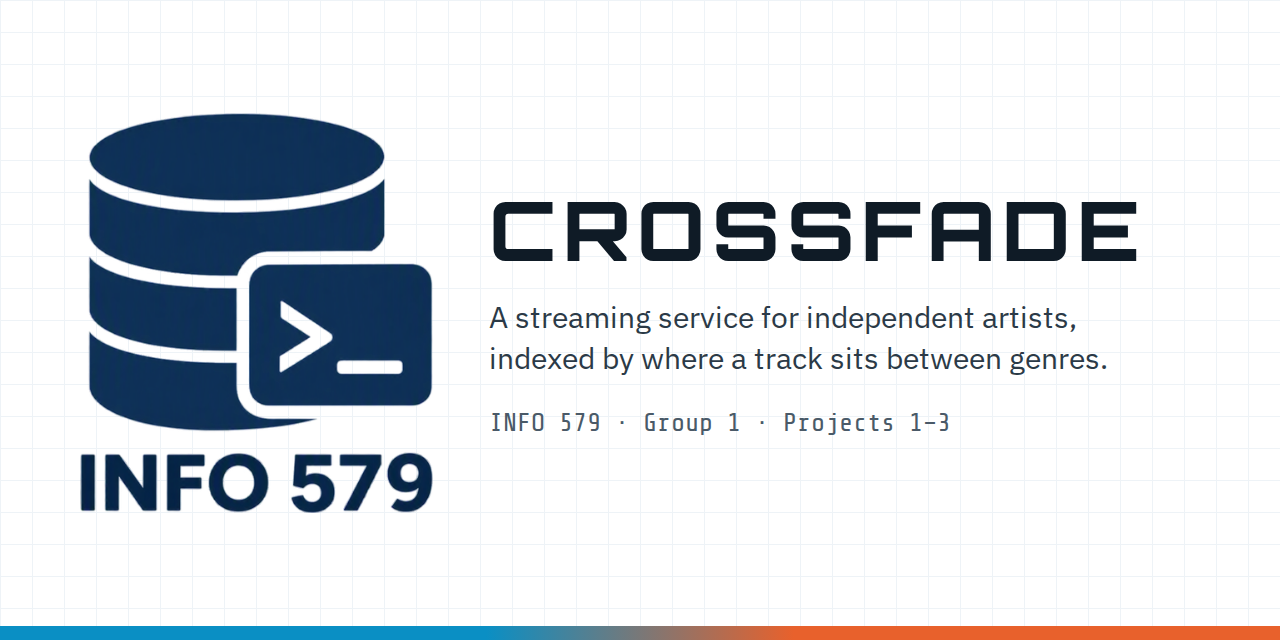
\includegraphics[width=1.75in]{og_crossfade.png} \\ \hline
BEARDOWN repository (INFO 510) & \url{https://github.com/N-Herling-Mk1/INFO_510_Fa25_Final_Proj} & \rule{0pt}{1.05in}
\includegraphics[height=0.95in]{og_beardown.png} \\ \hline
FORGE documentation (INFO 698) & \url{https://n-herling-mk1.github.io/INFO_698_documentation/} & \rule{0pt}{1.05in}
\includegraphics[width=1.75in]{og_forge_docs.png} \\ \hline
FORGE official website & \url{https://forge-observatory.com} & \rule{0pt}{1.05in}
\includegraphics[width=1.75in]{og_forge_site.png} \\ \hline
\end{longtable}}

\vspace{6pt}
\noindent\fcolorbox{headblue}{headblue!6}{\parbox{\dimexpr\linewidth-2\fboxsep-2\fboxrule}{%
\textbf{Data dictionary.} Every column in this document, 59 in all, is documented in the project's
data dictionary: its data type and size in bytes, the extreme or typical values in \texttt{data.xlsx},
why the type is the smallest correct choice, and what the column holds. Online at
\href{https://n-herling-mk1.github.io/INFO_579_Fa26_Proj1_CROSSFADE/project1/\#dictionary}{the CROSSFADE site, Data dictionary};
in the repository as \texttt{project1/docs/DATA\_DICTIONARY.md}. Each entity table in this document links to its section.}}

\clearpage
\section{Overview}\label{sec:ra}

CROSSFADE is a music streaming service for independent \rae{artists} in which the catalogue is indexed by where a \rae{recording} sits between \rae{genres} rather than by a single \rae{genre} label. \rae{Artists} upload their own \rae{recordings} directly and grant the service a streaming licence, which removes the need to negotiate rights with established labels and makes the catalogue consist almost entirely of new and obscure material. Every \rae{track} is passed through a machine learning \rae{scoring model} at the moment of ingest; the model returns a probability distribution across a fixed set of \rae{genres} together with measures of how uncertain and how internally inconsistent that distribution is. \rae{Listeners} do not browse by \rae{genre} name. They create \rae{stations} that describe a \rae{target blend}, for example sixty per cent jazz and forty per cent hip hop, together with a permitted range of ambiguity, and the service returns \rae{recordings} that genuinely occupy that region. Because a \rae{recording} is placed from its audio alone, a \rae{track} uploaded an hour ago is as recommendable as one with a million \rae{plays}, which is the operational advantage the service is built around. The database must therefore manage the \rae{artist} roster and its catalogue, the versioned \rae{scoring models}, \rae{the output each model produced for each track} and \rae{the probability it assigned to each genre}, \rae{listener} accounts and the \rae{stations} they define, and a record of every \rae{play} for the dual purpose of learning \rae{listener} taste and paying \rae{artists} their per stream royalty.

\subsection{Entities}
{\footnotesize\renewcommand{\arraystretch}{1.15}
\begin{longtable}{|L{0.25in}|L{1.75in}|L{0.62in}|L{3.68in}|}
\hline
\rowcolor{hdrgray}\textbf{\#} & \textbf{Entity (n=10)} & \textbf{Non-key attributes (n=38)} & \textbf{Attributes} \\ \hline
1 & \rae{Artist} & 5 & Artist ID (PK), Stage Name, Country, Joined Date, Payout Rate, Verified \\ \hline
2 & \rae{Track} & 5 & Track ID (PK), Artist ID (FK), Title, Duration, Release Date, Audio Checksum, Ingest Status \\ \hline
3 & \rae{Genre} & 2 & Genre ID (PK), Name, Description \\ \hline
4 & \rae{Listener} & 4 & Listener ID (PK), Email, Display Name, Plan Tier, Signup Date \\ \hline
5 & \rae{Scoring Model} & 7 & Model ID (PK), Version Label, Fusion Type, Embedding Dimension, Segment Length, Training Corpus, Holdout Accuracy, Deployed On \\ \hline
6 & \rae{Station} & 4 & Station ID (PK), Listener ID (FK), Model ID (FK), Name, Minimum Ambiguity, Maximum Ambiguity, Created On \\ \hline
7 & \rae{Track Score} {\small (associative)} & 5 & Track ID (PK, FK), Model ID (PK, FK), Genre ID (FK), Top Probability, Posterior Entropy, Model Divergence, Segment Variance, Scored On \\ \hline
8 & \rae{Play} {\small (associative)} & 4 & Listener ID (PK, FK), Track ID (PK, FK), Played At (PK), Station ID (FK, optional), Seconds Played, Completed, Reaction, Royalty Amount \\ \hline
9 & \rae{Station Blend} {\small (associative)} & 1 & Station ID (PK, FK), Genre ID (PK, FK), Weight \\ \hline
10 & \rae{Genre Probability} {\small (associative)} & 1 & Track ID (PK, FK), Model ID (PK, FK), Genre ID (PK, FK), Probability \\ \hline
\end{longtable}}
\vspace{-10pt}{\small The third column counts attributes, not records; it excludes primary key (PK) and foreign key (FK) attributes.}

\subsection{Relationships}
{\small\begin{multicols}{3}
\begin{itemize}[leftmargin=1.2em,itemsep=0pt,topsep=0pt]
  \item Artist 1:N Track
  \item Track M:N Scoring Model
  \item Genre 1:N Track Score
  \item Listener M:N Track
  \item Listener 1:N Station
  \item Scoring Model 1:N Station
  \item Station 1:N Play
  \item Station M:N Genre
  \item Track Score M:N Genre
\end{itemize}
\end{multicols}}

\clearpage
\section{Entities}\label{sec:entities}

\begin{entitytable}
\entityhead{Artist}{An independent musician or group that has registered with the service to upload recordings under a direct streaming licence, and is paid a per stream royalty on plays of those recordings. An artist may be registered before uploading a first recording.\dictnote{artist}{Artist}}
\attr{Artist ID}{MEDIUMINT UNSIGNED}{No}{Yes}{Yes}%
     {A unique identifier assigned to each artist when their registration is accepted, used to attribute catalogue and royalty records to that artist.}
\attr{Stage Name}{VARCHAR(64)}{No}{Yes}{No}%
     {The public performing name under which the artist releases material and appears throughout the listener-facing service.}
\attr{Country}{CHAR(2)}{Yes}{No}{No}%
     {The country in which the artist is based, recorded as its two-letter ISO 3166-1 code and used to determine which royalty payment channels and tax treatments apply.}
\attr{Joined Date}{DATE}{No}{No}{No}%
     {The date on which the artist's registration was accepted and their direct streaming licence took effect.}
\attr{Payout Rate}{DECIMAL(5,5)}{No}{No}{No}%
     {The amount in United States dollars the artist is paid for a single qualifying stream, negotiated at registration and fixed for the term of the licence. It is always below one dollar.}
\attr{Verified}{BIT(1)}{No}{No}{No}%
     {Whether the service has confirmed the artist's identity and their right to licence the material they upload.}
\end{entitytable}

\begin{entitytable}
\entityhead{Track}{A single audio recording uploaded by an artist, held in the catalogue and made available for streaming once it has been scored by at least one model. The audio file itself is held in an object store under a key computed from the Track ID, so no column stores its location.\dictnote{track}{Track}}
\attr{Track ID}{INT UNSIGNED}{No}{Yes}{Yes}%
     {A unique identifier assigned to each recording on upload, used to reference that recording across scoring and play records.}
\attr{Artist ID}{MEDIUMINT UNSIGNED}{No}{No}{No}%
     {Foreign key referencing Artist. The artist who uploaded the recording and to whom its royalties are paid.}
\attr{Title}{VARCHAR(128)}{No}{No}{No}%
     {The name of the recording as the artist wishes it to appear to listeners.}
\attr{Duration}{SMALLINT UNSIGNED}{No}{No}{No}%
     {The playing length of the recording in whole seconds, used to decide whether a play qualifies for royalty and to estimate station running time.}
\attr{Release Date}{DATE}{No}{No}{No}%
     {The date on which the recording became available to listeners, which may be later than the date it was uploaded.}
\attr{Audio Checksum}{BINARY(32)}{No}{Yes}{No}%
     {The SHA-256 digest of the audio file, used to detect duplicate uploads and to confirm that the stored file has not been altered since it was scored.}
\attr{Ingest Status}{ENUM(\q{awaiting scoring}, \q{scored}, \q{rejected})}{No}{No}{No}%
     {The stage the recording has reached in the upload pipeline: one of awaiting scoring, scored or rejected.}
\end{entitytable}

\begin{entitytable}
\entityhead{Genre}{One of the fixed set of musical categories over which every scoring model produces its probability distribution, forming the coordinate system in which listeners describe the blend they want.\dictnote{genre}{Genre}}
\attr{Genre ID}{TINYINT UNSIGNED}{No}{Yes}{Yes}%
     {A unique identifier for each genre in the fixed set, equal to the class index the scoring models output for that genre, so that a prediction is stored without translation and model output always refers to a controlled category rather than free text. The set is fixed at ten genres, assigned as follows: 0 blues, 1 classical, 2 country, 3 disco, 4 hiphop, 5 jazz, 6 metal, 7 pop, 8 reggae, 9 rock.}
\attr{Name}{VARCHAR(9)}{No}{Yes}{No}%
     {The label by which the genre is known to listeners, for example jazz, metal or reggae. The ten names are fixed by the scoring models' output classes; the longest, classical, has nine characters.}
\attr{Description}{VARCHAR(80)}{Yes}{No}{No}%
     {A short account of the musical characteristics the category covers, shown to listeners when they are composing a station blend, and kept to one line of 80 characters.}
\end{entitytable}

\begin{entitytable}
\entityhead{Listener}{A registered subscriber who streams recordings from the catalogue and defines the stations through which they discover new material.\dictnote{listener}{Listener}}
\attr{Listener ID}{INT UNSIGNED}{No}{Yes}{Yes}%
     {A unique identifier assigned to each subscriber at sign up, used to associate stations and play history with that subscriber.}
\attr{Email}{VARCHAR(254)}{No}{Yes}{No}%
     {The address used to sign in, to recover the account and to send billing correspondence.}
\attr{Display Name}{VARCHAR(32)}{No}{No}{No}%
     {The name the subscriber chooses to be shown by when a station they created is shared with other subscribers.}
\attr{Plan Tier}{ENUM(\q{free}, \q{standard}, \q{premium})}{No}{No}{No}%
     {The subscription level held by the listener, one of free, standard or premium, which determines the monthly charge and the limits placed on station creation and offline listening.}
\attr{Signup Date}{DATE}{No}{No}{No}%
     {The date on which the subscriber first registered, used to anchor the monthly billing cycle.}
\end{entitytable}

\begin{entitytable}
\entityhead{Scoring Model}{A specific trained and deployed version of the machine learning system that places recordings in genre space. Several versions are in service at once because they differ in architecture and therefore disagree with one another, and that disagreement is itself used as a signal.\dictnote{scoring-model}{Scoring Model}}
\attr{Model ID}{TINYINT UNSIGNED}{No}{Yes}{Yes}%
     {A unique identifier for each deployed model version, assigned in order of deployment starting at one, carried on every score so that no result is ever separated from the model that produced it.}
\attr{Version Label}{VARCHAR(32)}{No}{Yes}{No}%
     {The human readable release name of the model version, used in internal reporting and in the artist analytics product.}
\attr{Fusion Type}{ENUM(\q{concat}, \q{gated})}{No}{No}{No}%
     {The method by which the model combines its audio branch with its tabular branch, either concatenation (concat) or gated fusion (gated), which is one of the principal architectural differences between versions.}
\attr{Embedding Dimension}{SMALLINT UNSIGNED}{No}{No}{No}%
     {The width of the representation the model produces for a recording, which determines the geometry of the space in which similarity is measured.}
\attr{Segment Length}{TINYINT UNSIGNED}{No}{No}{No}%
     {The length in whole seconds of the audio window the model scores at a time; shorter windows allow a recording to be shown to shift in character across its own duration.}
\attr{Training Corpus}{VARCHAR(16)}{No}{No}{No}%
     {The name of the labelled collection the model version was trained on, recorded so that results from differently trained versions are never silently compared. Corpus names are short identifiers such as GTZAN; 16 characters covers the common public sets.}
\attr{Holdout Accuracy}{DECIMAL(5,4)}{No}{No}{No}%
     {The proportion of held out recordings the model version classified correctly, used to decide how much weight its output carries in a blended placement.}
\attr{Deployed On}{DATE}{No}{No}{No}%
     {The date the model version was placed in service and began scoring incoming uploads.}
\end{entitytable}

\begin{entitytable}
\entityhead{Station}{A standing description of a region of genre space created by a listener. A station stores the blend and the ambiguity range the listener wants rather than a fixed list of recordings, so its contents change as the catalogue grows.\dictnote{station}{Station}}
\attr{Station ID}{INT UNSIGNED}{No}{Yes}{Yes}%
     {A unique identifier for each station, used to record which station was responsible for surfacing a given play.}
\attr{Listener ID}{INT UNSIGNED}{No}{No}{No}%
     {Foreign key referencing Listener. The subscriber who created the station and to whose library it belongs.}
\attr{Model ID}{TINYINT UNSIGNED}{No}{No}{No}%
     {Foreign key referencing Scoring Model. The model version whose output the station is evaluated against.}
\attr{Name}{VARCHAR(64)}{No}{No}{No}%
     {The name the listener gives the station, which appears in their library and in any share link.}
\attr{Minimum Ambiguity}{DECIMAL(3,2)}{No}{No}{No}%
     {The lower bound, on the zero to one posterior entropy scale, on how unsettled a recording's placement must be to qualify; raising it excludes recordings that sit squarely inside a single genre. It may not exceed Maximum Ambiguity.}
\attr{Maximum Ambiguity}{DECIMAL(3,2)}{No}{No}{No}%
     {The upper bound, on the zero to one posterior entropy scale, on how unsettled a recording's placement may be; lowering it excludes recordings the models cannot place with any confidence.}
\attr{Created On}{DATE}{No}{No}{No}%
     {The date the listener created the station, used to order their library and to measure how long a station remains in use.}
\end{entitytable}

\clearpage
\section{Associative entities}\label{sec:assoc}

The primary key of each associative entity is formed from its foreign keys, the primary keys of
the entities it connects, and no associative entity has a surrogate key. Track Score, Station Blend
and Genre Probability follow that rule exactly, so each participates in two identifying
relationships. Genre Probability connects Track Score to Genre, so its key is the two-part key of
Track Score followed by Genre ID. Each key component is marked Unique = No, because a single
component repeats freely; only the combination is unique. Two of the associative entities also carry
a third relationship, which gives the model its two ternary structures: Track, Scoring Model and
Genre meet at Track Score, and Listener, Track and Station meet at Play. In both cases the third
foreign key stays outside the primary key. Genre ID is excluded because the top genre is determined
by the pair of recording and model, so adding it to the key would permit two top genres for one
pair. Station ID is excluded because it is optional, and a primary key column can never be empty.

Play follows the rule and adds exactly one column. Its foreign keys, Listener ID and Track ID, are
both in its key, but together they cannot identify a play, because a listener streams the same
recording many times. A surrogate Play ID would solve that only by abandoning the rule, which is
what the feedback on the first draft corrected. Played At, the moment the stream began, completes
the key instead. The course's own Unit 2 example uses the same pattern: in its student grades table,
student 12345678 takes Computing Mathematics in 2019 and again in 2020, so a grade is identified by
student and course only together with Year and Sem. The key is unique under two stated rules.
Played At is recorded in UTC, so a daylight-saving change can never repeat a time. A second event
with the same listener, recording and start time is a duplicate report of the same play, and the
key rejects it, which is what keeps a double-counted royalty out of the ledger.


\begin{entitytable}
\entityhead{Track Score}{The result one scoring model produced for one recording. This is the associative entity that resolves the many to many relationship between recordings and scoring models, and it is the parent record for every model output: the full genre distribution is held in Genre Probability rows that belong to it. No genre is ever recorded against a recording on its own, because a placement is a property of the pair of recording and model and not of the recording alone. The full distribution is held in Genre Probability; Genre ID, Top Probability, Posterior Entropy and Model Divergence are summaries derived from it and stored on this row so that stations can filter without reading ten rows per score. A result is written once, in the same transaction as its distribution, and is replaced whole on a rescore, so the stored summaries cannot drift from the distribution. The model's vector representation of the recording is held in a vector store under a key computed from the same Track ID and Model ID, so no column stores it.\dictnote{track-score}{Track Score}}
\attr{Track ID}{INT UNSIGNED}{No}{No}{Yes}%
     {Part of the composite primary key; foreign key referencing Track. The recording that was scored.}
\attr{Model ID}{TINYINT UNSIGNED}{No}{No}{Yes}%
     {Part of the composite primary key; foreign key referencing Scoring Model. The model version that produced the result. Together with Track ID it allows at most one result per recording and model; rescoring with the same version replaces that result, and a retrained model is deployed as a new version with its own Model ID.}
\attr{Genre ID}{TINYINT UNSIGNED}{No}{No}{No}%
     {Foreign key referencing Genre, not part of the primary key. The genre the model judged most likely for this recording; derived as the genre with the highest probability in Genre Probability for the same recording and model.}
\attr{Top Probability}{DECIMAL(5,4)}{No}{No}{No}%
     {The probability the model assigned to the genre it judged most likely, which is how confident that single placement is; derived as the largest probability in Genre Probability for the same recording and model.}
\attr{Posterior Entropy}{DECIMAL(5,4)}{No}{No}{No}%
     {How spread out the model's probability distribution is across all genres, expressed as the Shannon entropy divided by its maximum possible value so that it lies between zero and one; a high value means the recording sits between categories rather than inside one. Derived from the distribution in Genre Probability.}
\attr{Model Divergence}{DECIMAL(5,4)}{Yes}{No}{No}%
     {How far this model's distribution sits from those produced by the other model versions that have scored the same recording. It is the mean, over every other result for that recording, of the Jensen--Shannon divergence in base two between the two distributions; each divergence lies between zero and one, so the mean does too. It is empty while only one model has scored the recording, because there is nothing to compare against, and zero would wrongly claim perfect agreement. This is the cross model disagreement signal referred to in the Scoring Model definition. Derived from the distributions in Genre Probability; because it depends on the other models' results for the same recording, it is recomputed for every result of that recording whenever any model scores it.}
\attr{Segment Variance}{DECIMAL(4,4)}{Yes}{No}{No}%
     {How much the placement moves between one audio window and the next within the same recording, measured as the variance of the top genre probability across windows and therefore never above one quarter, which identifies tracks that change character partway through.}
\attr{Scored On}{DATETIME}{No}{No}{No}%
     {The moment the scoring run completed, used to establish which results predate a model redeployment and must be recomputed.}
\end{entitytable}

\begin{entitytable}
\entityhead{Play}{A single occasion on which a listener streamed a recording. This is the associative entity that resolves the many to many relationship between listeners and recordings, and it serves two purposes at once: it is the record from which listener taste is inferred and it is the billable event on which the artist royalty is calculated.\dictnote{play}{Play}}
\attr{Listener ID}{INT UNSIGNED}{No}{No}{Yes}%
     {Part of the composite primary key; foreign key referencing Listener. The subscriber who streamed the recording.}
\attr{Track ID}{INT UNSIGNED}{No}{No}{Yes}%
     {Part of the composite primary key; foreign key referencing Track. The recording that was streamed.}
\attr{Played At}{DATETIME}{No}{No}{Yes}%
     {Part of the composite primary key. The moment the stream began, recorded in UTC so that a daylight-saving change never repeats a value, and used to order listening history and to assign the play to a billing period. A listener may stream the same recording many times, so Listener ID and Track ID alone do not identify a play; the start time completes the key, and a repeated event with the same three values is rejected as a duplicate when the royalty ledger is reconciled.}
\attr{Station ID}{INT UNSIGNED}{Yes}{No}{No}%
     {Foreign key referencing Station, not part of the primary key. The station that surfaced the recording, left empty when the listener chose it directly. Because stations can be shared, the station may belong to a different listener from the one recorded on the play.}
\attr{Seconds Played}{SMALLINT UNSIGNED}{No}{No}{No}%
     {How much of the recording was actually streamed, which determines both whether the play qualifies for royalty and how strong a taste signal it carries.}
\attr{Completed}{BIT(1)}{No}{No}{No}%
     {Whether the listener heard the recording to its end, distinguishing a genuine listen from an abandoned one. Derived: true exactly when Seconds Played equals the Duration of the recording. It is stored so that listening history can be filtered to finished plays without a join to Track, and it is set only by the procedure that records the play (I7).}
\attr{Reaction}{ENUM(\q{saved}, \q{skipped})}{Yes}{No}{No}%
     {An explicit response from the listener where one was given, either saved or skipped, which is treated as a stronger signal than duration alone.}
\attr{Royalty Amount}{DECIMAL(5,5)}{No}{No}{No}%
     {The amount in United States dollars accrued to the artist for this play. A snapshot rather than a derived value: it is the artist's Payout Rate as it stood at the time of a qualifying play of 30 seconds or more, and zero otherwise, copied so that a later rate change never rewrites the royalty ledger (I7).}
\end{entitytable}

\begin{entitytable}
\entityhead{Station Blend}{The weight one station gives to one genre. This is the associative entity that resolves the many to many relationship between stations and genres: a station blends several genres and a genre appears in many stations. Holding one weight per row keeps every value atomic, which a single multi-valued blend field on the station could not.\dictnote{station-blend}{Station Blend}}
\attr{Station ID}{INT UNSIGNED}{No}{No}{Yes}%
     {Part of the composite primary key; foreign key referencing Station. The station whose blend this row belongs to.}
\attr{Genre ID}{TINYINT UNSIGNED}{No}{No}{Yes}%
     {Part of the composite primary key; foreign key referencing Genre. The genre being weighted. Together with Station ID it allows at most one weight per genre in a station, so a single weight can be adjusted without rewriting the rest of the blend.}
\attr{Weight}{DECIMAL(3,2)}{No}{No}{No}%
     {The share of the station's blend given to this genre, greater than zero and at most one. The weights belonging to one station sum to exactly 1.00; because this is a rule across rows, it is enforced when the blend is written (see Integrity rules), not by a single-row check.}
\end{entitytable}

\begin{entitytable}
\entityhead{Genre Probability}{The probability one scoring model assigned to one genre for one recording. This is the associative entity that resolves the many to many relationship between scoring results and genres: a result assigns a probability to every genre, and a genre receives a probability in every result. It holds the full distribution that stations match against, which the single top genre on Track Score cannot express.\dictnote{genre-probability}{Genre Probability}}
\attr{Track ID}{INT UNSIGNED}{No}{No}{Yes}%
     {Part of the composite primary key. Together with Model ID it forms a composite foreign key referencing Track Score, so a probability can only be recorded for a recording and model pair that has a scoring result.}
\attr{Model ID}{TINYINT UNSIGNED}{No}{No}{Yes}%
     {Part of the composite primary key and of the composite foreign key referencing Track Score. The model version that produced the distribution.}
\attr{Genre ID}{TINYINT UNSIGNED}{No}{No}{Yes}%
     {Part of the composite primary key; foreign key referencing Genre. The genre this probability belongs to.}
\attr{Probability}{DECIMAL(5,4)}{No}{No}{No}%
     {The probability, between zero and one, that the model assigned to this genre for this recording. The ten probabilities of one result sum to one, within rounding.}
\end{entitytable}

\Needspace{10\baselineskip}
\section{Relationships}\label{sec:rels}

\begin{longtable}{|L{1.15in}|L{1.15in}|L{0.9in}|L{3.05in}|}
\hline
\rowcolor{hdrgray}\textbf{Parent} & \textbf{Child} & \textbf{Cardinality} & \textbf{Description} \\ \hline
\endfirsthead
\hline
\rowcolor{hdrgray}\textbf{Parent} & \textbf{Child} & \textbf{Cardinality} & \textbf{Description} \\ \hline
\endhead
Artist & Track & 1:N & An artist contributes zero or more recordings to the catalogue (none between registration and the first upload), and every recording belongs to exactly one artist, who is the party the royalty is paid to. \\ \hline
Track & Scoring Model & M:N & A recording is scored by zero or more model versions (none while it is awaiting scoring, at least one before it is released) and a model version scores many recordings. The relationship is resolved by the associative entity Track Score, whose primary key is Track ID and Model ID. \\ \hline
Genre & Track Score & 1:N & Each scoring result names the single genre the model judged most likely, and one genre is named by many scoring results. The genre is recorded on the result, as a foreign key outside the primary key, and never on the recording itself. \\ \hline
Listener & Track & M:N & A listener streams many recordings and a recording is streamed by many listeners. The relationship is resolved by the associative entity Play, whose primary key is Listener ID, Track ID and Played At. \\ \hline
Listener & Station & 1:N & A listener creates zero or more stations and every station belongs to exactly one listener. \\ \hline
Scoring Model & Station & 1:N & Each station is evaluated against the output of one nominated model version, so that a station's contents do not change meaning when a different version scores the catalogue. One model version serves many stations. \\ \hline
Station & Play & 1:N & A station is responsible for many streaming events, while a play may have arisen from a station or from the listener choosing a recording directly, in which case Station ID on the play is left empty. A station may be shared, so it can surface plays for listeners other than its creator. \\ \hline
Station & Genre & M:N & A station blends one or more genres and a genre appears in many stations. The relationship is resolved by the associative entity Station Blend, whose primary key is Station ID and Genre ID. \\ \hline
Track Score & Genre & M:N & A scoring result assigns a probability to every genre and a genre receives a probability in every result. The relationship is resolved by the associative entity Genre Probability, whose primary key is Track ID, Model ID and Genre ID. \\ \hline
\end{longtable}

\subsection{Integrity rules}\label{sec:integ}
Keys and single-row checks cannot express every rule. The rules below span rows or tables. Each is
enforced by a stored procedure that writes all the affected rows in one transaction and either computes
the dependent values itself or validates them before it commits. A transaction alone guarantees only
that the rows are written together, not that they agree, so the procedures do not accept derived
values as input. The application account is granted EXECUTE on these procedures and no direct INSERT,
UPDATE or DELETE on Track Score, Genre Probability or Station Blend, so the procedures are the only
write path to those tables.

\begin{longtable}{|L{0.35in}|L{2.55in}|L{3.30in}|}
\hline
\rowcolor{hdrgray}\textbf{\#} & \textbf{Rule} & \textbf{Enforcement} \\ \hline
\endfirsthead
\hline
\rowcolor{hdrgray}\textbf{\#} & \textbf{Rule} & \textbf{Enforcement} \\ \hline
\endhead
I1 & A station has at least one blend row, and its weights sum to exactly 1.00. & The procedure that saves a blend replaces all of the station's rows at once and rolls back unless there is at least one row and SUM(Weight) = 1.00. A station and its first blend are created in the same call. Weights are held in hundredths, so a three-genre blend is stored as 0.34, 0.33 and 0.33, never as three equal thirds. \\ \hline
I2 & A scoring result has exactly one probability for each of the ten genres, and they sum to one. & The scoring procedure takes the ten probabilities as its input and rolls back unless there are exactly as many rows as there are Genre records, one per genre, summing to one within 0.0010, the rounding allowance for ten values held to four decimal places. \\ \hline
I3 & Genre ID, Top Probability, Posterior Entropy and Model Divergence on Track Score agree with the probabilities in Genre Probability. & The scoring procedure computes all four from the probability rows it has just written rather than accepting them as input: the most likely genre, its probability, the normalised Shannon entropy, and the mean base-two Jensen--Shannon divergence against every other result for the same recording, left empty when there is no other result. Because divergence depends on those other results, the procedure recomputes it for all of the recording's results. A rescore replaces the result and its distribution together. \\ \hline
I4 & Minimum Ambiguity does not exceed Maximum Ambiguity. & A single-row CHECK constraint on Station. \\ \hline
I5 & A recording's Ingest Status is scored only if it has at least one Track Score. & Set in the scoring transaction that inserts the first result. \\ \hline
I6 & A play's Station ID may refer to a station created by another listener. & Deliberately not constrained by the database: stations can be shared, so the station's Listener ID need not match the play's. Whether a listener may use a given station is a sharing permission checked by the application. \\ \hline
I7 & Completed is true exactly when Seconds Played equals the recording's Duration, and Royalty Amount equals the artist's Payout Rate for a play of 30 seconds or more and zero otherwise. & The procedure that records a play computes both from the Track and Artist rows rather than accepting them as input, as I3 does for Track Score. Royalty Amount is computed once, when the play is recorded, and never updated. \\ \hline
\end{longtable}

\clearpage

\section{Index and Colour Coding}\label{sec:index}

Every entity, associative entity and relationship in the requirements analysis, colour coded by kind.
The same colour marks a name wherever it appears in these tables.

\swatch{entc}\ \ent{Entity}\qquad
\swatch{ascc}\ \asc{Associative entity}\qquad
\swatch{relc}\ \rel{Relationship}

\begin{longtable}{|L{0.35in}|L{1.25in}|L{0.80in}|L{1.05in}|T{1.30in}|L{1.20in}|}
\hline
\rowcolor{entbg}\multicolumn{6}{|l|}{\cellcolor{entbg}\textcolor{entc}{\textbf{Table 1 --- Entities (6)}}\label{tab:ent}} \\ \hline
\rowcolor{hdrgray}\textbf{\#} & \textbf{Name} & \textbf{Attributes} & \textbf{Primary Key} & \textbf{Key Type} & \textbf{Example} \\ \hline
E1 & \ent{Artist} & 5 & Artist ID & MEDIUMINT UNSIGNED & 1042 (Velvet Static) \\ \hline
E2 & \ent{Track} & 5 & Track ID & INT UNSIGNED & 4817 (Low Tide Signal) \\ \hline
E3 & \ent{Genre} & 2 & Genre ID & TINYINT UNSIGNED & 5 (jazz) \\ \hline
E4 & \ent{Listener} & 4 & Listener ID & INT UNSIGNED & 20931 (jrivera) \\ \hline
E5 & \ent{Scoring Model} & 7 & Model ID & TINYINT UNSIGNED & 5 (beardown\_3sec) \\ \hline
E6 & \ent{Station} & 4 & Station ID & INT UNSIGNED & 7710 (Late Jazz Hop) \\ \hline
\end{longtable}

Genre ID and Model ID are the only keys whose values are fixed by the design rather than
generated. Each value below is one record of the Genre or Scoring Model table; child tables
store only the number, and a join on the key returns the name. Genre ID equals the class
index the scoring models output. Model ID is assigned in order of deployment.

\begin{longtable}{|L{1.30in}|L{0.80in}|L{2.00in}|L{2.20in}|}
\hline
\rowcolor{entbg}\multicolumn{4}{|l|}{\cellcolor{entbg}\textcolor{entc}{\textbf{Table 2 --- Key reference for controlled keys}}\label{tab:keys}} \\ \hline
\rowcolor{hdrgray}\textbf{Key} & \textbf{Value} & \textbf{Name} & \textbf{Source} \\ \hline
\ent{Genre} ID & 0 & blues & model class index \\ \hline
\ent{Genre} ID & 1 & classical & model class index \\ \hline
\ent{Genre} ID & 2 & country & model class index \\ \hline
\ent{Genre} ID & 3 & disco & model class index \\ \hline
\ent{Genre} ID & 4 & hiphop & model class index \\ \hline
\ent{Genre} ID & 5 & jazz & model class index \\ \hline
\ent{Genre} ID & 6 & metal & model class index \\ \hline
\ent{Genre} ID & 7 & pop & model class index \\ \hline
\ent{Genre} ID & 8 & reggae & model class index \\ \hline
\ent{Genre} ID & 9 & rock & model class index \\ \hline
\ent{Scoring Model} ID & 1 & beardown & deployment order \\ \hline
\ent{Scoring Model} ID & 2 & beardown\_rrm\_cfg12 & deployment order \\ \hline
\ent{Scoring Model} ID & 3 & beardown\_rrm\_cfg17 & deployment order \\ \hline
\ent{Scoring Model} ID & 4 & beardown\_rrm & deployment order \\ \hline
\ent{Scoring Model} ID & 5 & beardown\_3sec & deployment order \\ \hline
\end{longtable}

\begin{longtable}{|L{0.40in}|L{1.30in}|L{0.85in}|L{2.05in}|L{1.60in}|}
\hline
\rowcolor{ascbg}\multicolumn{5}{|l|}{\cellcolor{ascbg}\textcolor{ascc}{\textbf{Table 3 --- Associative entities (4)}}\label{tab:asc}} \\ \hline
\rowcolor{hdrgray}\textbf{\#} & \textbf{Name} & \textbf{Attributes} & \textbf{Primary Key} & \textbf{Resolves} \\ \hline
A1 & \asc{Track Score} & 5 & Track ID + Model ID & \ent{Track} M:N \ent{Scoring Model} (R2) \\ \hline
A2 & \asc{Play} & 4 & Listener ID + Track ID + Played At & \ent{Listener} M:N \ent{Track} (R4) \\ \hline
A3 & \asc{Station Blend} & 1 & Station ID + Genre ID & \ent{Station} M:N \ent{Genre} (R8) \\ \hline
A4 & \asc{Genre Probability} & 1 & Track ID + Model ID + Genre ID & \asc{Track Score} M:N \ent{Genre} (R9) \\ \hline
\end{longtable}

\begin{longtable}{|L{0.40in}|L{1.45in}|L{1.45in}|L{0.95in}|L{1.85in}|}
\hline
\rowcolor{relbg}\multicolumn{5}{|l|}{\cellcolor{relbg}\textcolor{relc}{\textbf{Table 4 --- Relationships (9)}}\label{tab:rel}} \\ \hline
\rowcolor{hdrgray}\textbf{\#} & \textbf{Parent} & \textbf{Child} & \textbf{Cardinality} & \textbf{Resolved by} \\ \hline
\rel{R1} & \ent{Artist} & \ent{Track} & 1:N & --- \\ \hline
\rel{R2} & \ent{Track} & \ent{Scoring Model} & \textbf{M:N} & \asc{Track Score} \\ \hline
\rel{R3} & \ent{Genre} & \asc{Track Score} & 1:N & --- \\ \hline
\rel{R4} & \ent{Listener} & \ent{Track} & \textbf{M:N} & \asc{Play} \\ \hline
\rel{R5} & \ent{Listener} & \ent{Station} & 1:N & --- \\ \hline
\rel{R6} & \ent{Scoring Model} & \ent{Station} & 1:N & --- \\ \hline
\rel{R7} & \ent{Station} & \asc{Play} & 1:N & --- \\ \hline
\rel{R8} & \ent{Station} & \ent{Genre} & \textbf{M:N} & \asc{Station Blend} \\ \hline
\rel{R9} & \asc{Track Score} & \ent{Genre} & \textbf{M:N} & \asc{Genre Probability} \\ \hline
\end{longtable}

\begin{longtable}{|L{1.00in}|L{1.90in}|L{1.20in}|L{2.15in}|}
\hline
\rowcolor{relbg}\multicolumn{4}{|l|}{\cellcolor{relbg}\textcolor{relc}{\textbf{Table 5 --- Resolution of each many-to-many relationship}}\label{tab:res}} \\ \hline
\rowcolor{hdrgray}\textbf{Relationship} & \textbf{Before} & \textbf{Via} & \textbf{After} \\ \hline
\rel{R2} & \ent{Track} M:N \ent{Scoring Model} & \asc{Track Score} & \ent{Track} 1:N \asc{Track Score} \\ \hline
 & & & \ent{Scoring Model} 1:N \asc{Track Score} \\ \hline
\rel{R4} & \ent{Listener} M:N \ent{Track} & \asc{Play} & \ent{Listener} 1:N \asc{Play} \\ \hline
 & & & \ent{Track} 1:N \asc{Play} \\ \hline
\rel{R8} & \ent{Station} M:N \ent{Genre} & \asc{Station Blend} & \ent{Station} 1:N \asc{Station Blend} \\ \hline
 & & & \ent{Genre} 1:N \asc{Station Blend} \\ \hline
\rel{R9} & \asc{Track Score} M:N \ent{Genre} & \asc{Genre Probability} & \asc{Track Score} 1:N \asc{Genre Probability} \\ \hline
 & & & \ent{Genre} 1:N \asc{Genre Probability} \\ \hline
\end{longtable}

\Needspace{20\baselineskip}
Every foreign key in the design, with the relationship it implements. A foreign key that is part of
its owner's primary key implements an identifying relationship; one that is not implements a
non-identifying relationship.

\begin{longtable}{|L{1.15in}|L{1.00in}|L{1.10in}|L{0.55in}|L{0.40in}|L{1.70in}|}
\hline
\rowcolor{relbg}\multicolumn{6}{|l|}{\cellcolor{relbg}\textcolor{relc}{\textbf{Table 6 --- Foreign keys (14 columns)}}\label{tab:fk}} \\ \hline
\rowcolor{hdrgray}\textbf{Owner} & \textbf{Foreign key} & \textbf{References} & \textbf{In PK} & \textbf{Rel.} & \textbf{Relationship type} \\ \hline
\ent{Track} & Artist ID & \ent{Artist} & No & \rel{R1} & non-identifying \\ \hline
\ent{Station} & Listener ID & \ent{Listener} & No & \rel{R5} & non-identifying \\ \hline
\ent{Station} & Model ID & \ent{Scoring Model} & No & \rel{R6} & non-identifying \\ \hline
\asc{Track Score} & Track ID & \ent{Track} & Yes & \rel{R2} & identifying \\ \hline
\asc{Track Score} & Model ID & \ent{Scoring Model} & Yes & \rel{R2} & identifying \\ \hline
\asc{Track Score} & Genre ID & \ent{Genre} & No & \rel{R3} & non-identifying \\ \hline
\asc{Play} & Listener ID & \ent{Listener} & Yes & \rel{R4} & identifying \\ \hline
\asc{Play} & Track ID & \ent{Track} & Yes & \rel{R4} & identifying \\ \hline
\asc{Play} & Station ID & \ent{Station} & No & \rel{R7} & non-identifying, optional \\ \hline
\asc{Station Blend} & Station ID & \ent{Station} & Yes & \rel{R8} & identifying \\ \hline
\asc{Station Blend} & Genre ID & \ent{Genre} & Yes & \rel{R8} & identifying \\ \hline
\asc{Genre Probability} & Track ID + Model ID & \asc{Track Score} & Yes & \rel{R9} & identifying, composite \\ \hline
\asc{Genre Probability} & Genre ID & \ent{Genre} & Yes & \rel{R9} & identifying \\ \hline
\end{longtable}

\clearpage
\section{Document Inventory}\label{sec:inv}

Everything this document currently contains, followed by the evidence that the design meets
each stated design requirement, a full attribute inventory and the data types used.

\begin{longtable}{|L{4.60in}|L{1.00in}|}
\hline
\rowcolor{hdrgray}\multicolumn{2}{|l|}{\cellcolor{hdrgray}\textbf{Contents}} \\ \hline
\rowcolor{hdrgray}\textbf{Item} & \textbf{Page} \\ \hline
Background, with BEARDOWN and FORGE links & \pageref{sec:bg} \\ \hline
Overview, with entity and relationship lists & \pageref{sec:ra} \\ \hline
Entities (6) & \pageref{sec:entities} \\ \hline
Associative entities (4) & \pageref{sec:assoc} \\ \hline
Relationships (9) & \pageref{sec:rels} \\ \hline
\quad Integrity rules & \pageref{sec:integ} \\ \hline
Index and colour coding & \pageref{sec:index} \\ \hline
\quad Table 1 --- Entities & \pageref{tab:ent} \\ \hline
\quad Table 2 --- Key reference for controlled keys & \pageref{tab:keys} \\ \hline
\quad Table 3 --- Associative entities & \pageref{tab:asc} \\ \hline
\quad Table 4 --- Relationships & \pageref{tab:rel} \\ \hline
\quad Table 5 --- Resolution of each many-to-many relationship & \pageref{tab:res} \\ \hline
\quad Table 6 --- Foreign keys & \pageref{tab:fk} \\ \hline
Document inventory & \pageref{sec:inv} \\ \hline
\quad Table 7 --- Design requirement checks & \pageref{tab:chk} \\ \hline
\quad Table 8 --- Attribute inventory & \pageref{tab:attr} \\ \hline
\quad Table 9 --- Data types used, by family & \pageref{tab:types} \\ \hline
\end{longtable}

\begin{longtable}{|L{2.20in}|L{0.75in}|L{0.95in}|L{0.70in}|L{1.45in}|}
\hline
\rowcolor{hdrgray}\multicolumn{5}{|l|}{\cellcolor{hdrgray}\textbf{Table 7 --- Design requirement checks}\label{tab:chk}} \\ \hline
\rowcolor{hdrgray}\textbf{Requirement} & \textbf{Required} & \textbf{This design} & \textbf{Status} & \textbf{Evidence} \\ \hline
Non-associative entities & 5 to 7 & 6 & \textcolor{relc}{\textbf{Met}} & Table 1 \\ \hline
Attributes, excluding primary and foreign keys & $\geq$ 20 & 38 & \textcolor{relc}{\textbf{Met}} & Table 8 \\ \hline
Many-to-many relationships resolved with an associative entity & $\geq$ 1 & 4 & \textcolor{relc}{\textbf{Met}} & Tables 3, 4, 5, 6 \\ \hline
\end{longtable}

\textbf{Requirement 1.} The design has 6 non-associative entities (Table 1). The 4
associative entities are listed separately (Table 3) and are not counted.

\textbf{Requirement 2.} The design has 38 attributes excluding primary and foreign keys:
27 on the entities and 11 on the associative entities. Primary keys (Tables 1 and 3) and the
14 foreign key columns (Table 6) are not counted. Played At is counted as part of Play's primary key
and is therefore excluded as well, although it is not a foreign key.

\textbf{Requirement 4.} Four of the nine relationships are many-to-many (Table 4), each resolved by
an associative entity (Table 3) into two one-to-many identifying relationships (Table 5). Each key is
formed from the keys of the entities it connects (Table 6); Play's also includes Played At.

Table 8 lists every attribute on its own row with its data type, the range that type
admits and an example value. Scoring Model values are those of a real deployed version, the
3-second segment model trained on GTZAN; the remaining values are illustrative, with the
Track Score figures computed from one example posterior so that they agree with one another
and fall inside the example station's ambiguity range.

{\setlength{\tabcolsep}{4pt}\small
\begin{longtable}{|L{0.28in}|L{1.00in}|L{1.30in}|T{1.35in}|L{1.15in}|L{1.20in}|}
\hline
\rowcolor{hdrgray}\multicolumn{6}{|l|}{\cellcolor{hdrgray}\textbf{Table 8 --- Attribute inventory (38)}\label{tab:attr}} \\ \hline
\rowcolor{hdrgray}\textbf{\#} & \textbf{Owner} & \textbf{Attribute} & \textbf{Data Type} & \textbf{Range} & \textbf{Example} \\ \hline
\endfirsthead
\hline
\rowcolor{hdrgray}\textbf{\#} & \textbf{Owner} & \textbf{Attribute} & \textbf{Data Type} & \textbf{Range} & \textbf{Example} \\ \hline
\endhead
1 & \ent{Artist} & Stage Name & VARCHAR(64) & up to 64 characters & Velvet Static \\ \hline
2 & \ent{Artist} & Country & CHAR(2) & ISO 3166-1 alpha-2 code & US \\ \hline
3 & \ent{Artist} & Joined Date & DATE & calendar date & 2026-03-14 \\ \hline
4 & \ent{Artist} & Payout Rate & DECIMAL(5,5) & 0.00000 to 0.99999 USD & 0.00400 \\ \hline
5 & \ent{Artist} & Verified & BIT(1) & 0 or 1 & 1 \\ \hline
6 & \ent{Track} & Title & VARCHAR(128) & up to 128 characters & Low Tide Signal \\ \hline
7 & \ent{Track} & Duration & SMALLINT UNSIGNED & 0 to 65,535 s & 214 \\ \hline
8 & \ent{Track} & Release Date & DATE & calendar date & 2026-04-02 \\ \hline
9 & \ent{Track} & Audio Checksum & BINARY(32) & 32-byte SHA-256 digest & 0x9F3A\ldots C21E \\ \hline
10 & \ent{Track} & Ingest Status & ENUM(\q{awaiting scoring}, \q{scored}, \q{rejected}) & one of 3 values & \q{scored} \\ \hline
11 & \ent{Genre} & Name & VARCHAR(9) & one of 10 names, longest \q{classical} (9) & jazz \\ \hline
12 & \ent{Genre} & Description & VARCHAR(80) & up to 80 characters & Swing, improvisation and extended harmony \\ \hline
13 & \ent{Listener} & Email & VARCHAR(254) & up to 254 characters & j.rivera@\allowbreak example.com \\ \hline
14 & \ent{Listener} & Display Name & VARCHAR(32) & up to 32 characters & jrivera \\ \hline
15 & \ent{Listener} & Plan Tier & ENUM(\q{free}, \q{standard}, \q{premium}) & one of 3 values & \q{standard} \\ \hline
16 & \ent{Listener} & Signup Date & DATE & calendar date & 2026-05-09 \\ \hline
17 & \ent{Scoring Model} & Version Label & VARCHAR(32) & up to 32 characters & beardown\_3sec \\ \hline
18 & \ent{Scoring Model} & Fusion Type & ENUM(\q{concat}, \q{gated}) & one of 2 values & \q{concat} \\ \hline
19 & \ent{Scoring Model} & Embedding Dimension & SMALLINT UNSIGNED & 0 to 65,535 & 384 \\ \hline
20 & \ent{Scoring Model} & Segment Length & TINYINT UNSIGNED & 0 to 255 s & 3 \\ \hline
21 & \ent{Scoring Model} & Training Corpus & VARCHAR(16) & up to 16 characters & GTZAN \\ \hline
22 & \ent{Scoring Model} & Holdout Accuracy & DECIMAL(5,4) & 0.0000 to 1.0000 & 0.7887 \\ \hline
23 & \ent{Scoring Model} & Deployed On & DATE & calendar date & 2026-06-23 \\ \hline
24 & \ent{Station} & Name & VARCHAR(64) & up to 64 characters & Late Jazz Hop \\ \hline
25 & \ent{Station} & Minimum Ambiguity & DECIMAL(3,2) & 0.00 to 1.00 & 0.35 \\ \hline
26 & \ent{Station} & Maximum Ambiguity & DECIMAL(3,2) & 0.00 to 1.00 & 0.80 \\ \hline
27 & \ent{Station} & Created On & DATE & calendar date & 2026-08-01 \\ \hline
28 & \asc{Track Score} & Top Probability & DECIMAL(5,4) & 0.0000 to 1.0000 & 0.5800 \\ \hline
29 & \asc{Track Score} & Posterior Entropy & DECIMAL(5,4) & 0.0000 to 1.0000 & 0.4619 \\ \hline
30 & \asc{Track Score} & Model Divergence & DECIMAL(5,4) & 0.0000 to 1.0000, or empty & 0.0198 \\ \hline
31 & \asc{Track Score} & Segment Variance & DECIMAL(4,4) & 0.0000 to 0.2500 & 0.0051 \\ \hline
32 & \asc{Track Score} & Scored On & DATETIME & date and time & 2026-07-01 09:14:52 \\ \hline
33 & \asc{Play} & Seconds Played & SMALLINT UNSIGNED & 0 to 65,535 s & 214 \\ \hline
34 & \asc{Play} & Completed & BIT(1) & 0 or 1 & 1 \\ \hline
35 & \asc{Play} & Reaction & ENUM(\q{saved}, \q{skipped}) & one of 2 values & \q{saved} \\ \hline
36 & \asc{Play} & Royalty Amount & DECIMAL(5,5) & 0.00000 to 0.99999 USD & 0.00400 \\ \hline
37 & \asc{Station Blend} & Weight & DECIMAL(3,2) & 0.01 to 1.00 & 0.60 \\ \hline
38 & \asc{Genre Probability} & Probability & DECIMAL(5,4) & 0.0000 to 1.0000 & 0.5800 \\ \hline
\end{longtable}}

\Needspace{34\baselineskip}
Every data type in this document is taken from the MySQL type set presented in the Unit 4
slides, and each column is given the smallest type whose range covers every value the
attribute can legitimately hold. Integer keys are declared unsigned because no identifier
is negative. Strings follow four rules. A value whose length never varies is CHAR (Country) or
BINARY (Audio Checksum), which saves VARCHAR's length byte. A value drawn from a closed
set gets a VARCHAR sized to its longest member: Genre Name is one of ten fixed names, the
longest nine. A value that can be computed from other columns is not stored at all: the
object-store key of a recording's audio and the vector-store key of a model's representation
are both computed from the primary key, so neither has a column. Free text entered by people (names, titles, email) gets a ceiling set by policy or
standard, since VARCHAR stores only the characters used plus a length byte. Ranges that a type cannot enforce on its own, such as a probability lying
between zero and one, are stated in the attribute description and are enforced in the
physical model with CHECK constraints. Two types from the slides are deliberately not used:
TIMESTAMP, whose range ends in January 2038, well within the life of a royalty ledger, so
DATETIME is used for moments in time. That is the one place parsimony is knowingly traded:
the slides give DATETIME 8 bytes against TIMESTAMP's 4 (MySQL 5.6.4 and later stores DATETIME
in 5), and Played At is part of Play's key, but a play recorded after 2038 must still be payable. FLOAT and DOUBLE are not used either, because every fractional value
here has a known precision and DECIMAL stores it exactly.

\begin{longtable}{|L{1.10in}|T{2.50in}|L{0.70in}|L{1.98in}|}
\hline
\rowcolor{hdrgray}\multicolumn{4}{|l|}{\cellcolor{hdrgray}\textbf{Table 9 --- Data types used, by family}\label{tab:types}} \\ \hline
\rowcolor{hdrgray}\textbf{Family} & \textbf{Types used} & \textbf{Columns} & \textbf{Slide source} \\ \hline
Integer & INT UNSIGNED, MEDIUMINT UNSIGNED, SMALLINT UNSIGNED, TINYINT UNSIGNED & 24 & Unit 4, Numeric Data Types \\ \hline
Fixed-point & DECIMAL(3,2), DECIMAL(4,4), DECIMAL(5,4), DECIMAL(5,5) & 11 & Unit 4, Numeric Data Types \\ \hline
String & CHAR(2), VARCHAR(9), VARCHAR(16), VARCHAR(32), VARCHAR(64), VARCHAR(80), VARCHAR(128), VARCHAR(254) & 10 & Unit 4, String Data Types \\ \hline
Binary & BINARY(32) & 1 & Unit 4, Binary Data Types \\ \hline
Date and time & DATE, DATETIME & 7 & Unit 4, Date and Time Types \\ \hline
Enumeration & ENUM (4 definitions) & 4 & Unit 4, Other Data Types \\ \hline
Boolean & BIT(1) & 2 & Unit 4, Other Data Types \\ \hline
\end{longtable}

\end{document}